\documentclass[../main.tex]{subfiles}
\graphicspath{{\subfix{../images/}}}
\begin{document}

\section{Introduction}
La théorie de la complexité est le domaine des mathématiques qui étudie le temps de calcul et la mémoire nécessaire par un ordinateur pour résoudre un
problème algorithmique (un problème qui peut être résolu avec un algorithme). Les algorithmes qui résolvent le problème sont évalués selon des critères
pour trouver celui l'algorithme le plus optimale (et approprié) avec les ressources disponibles. Dans un premier temps les définitions de ces critères sera
présentée. Dans un autre temps, la notion de classification des problèmes sera introduite; les problèmes sont classés selon leur \og difficulté \fg{} à
résoudre à l'aide d'un algorithme.

\section{Définitions}
\subsection{Complexité en temps}
La complexité en temps est une des notions les plus importantes dans la théorie de la complexité. Les notations grand O de Landau sont utilisées pour évaluer
le temps nécessaire pour résoudre un problème. On définit la notation $O(f(n))$ avec $f(n)$ comme variable discrète et $n$ la taille des entrées
pour voir la croissance du nombre d'opérations maximum (et par la suite, le temps maximum pris pour résoudre le problème) quand $n\to\infty$.
Seulement le terme le plus important (le terme qui croit le plus rapidement) est pris en considération, sans son coefficient.
Un algorithme $f(n)$ est résolu dans un temps polynomial quand $f(n)=O(n^k)$ pour $k \in \mathbb{Z}^+$ et quand $n\to\infty$. Quand un algorithme résout le problème dans un temps polynomial ou moins (logarithmique), il est considéré comme un algorithme rapide.

Par exemple, 2 algorithmes sont utilisés pour chercher un mot dans un dictionnaire de taille $n$ mots. Le premier compare les mots par ordre alphabétique jusqu'à trouver le mot désiré. L'autre est l'algorithme de recherche dichotomique (\emph{binary search} en anglais): il divise l'ensemble des mots en 2 parties égaux évalue dans quelle sous-ensemble le mot appartient (selon l'ordre alphabétique) et recommence la première étape avec le sous-ensemble (redivise le sous-ensemble en 2) jusqu'à trouver le mot dans le dictionnaire. Le premier prends $n$ étapes au pire des cas (le mot cherché est le dernier mot dans le dictionnaire), il est donc d'ordre $O(n)$. La recherche dichotomique est d'ordre $O(\log n)$. Par la suite la recherche dichotomique est plus optimale pour chercher un mot dans un dictionnaire.

Les ordres de grandeur les plus communs sont les suivants: $O(1)$ pour ordre constant, $O(\log n)$ pour ordre logarithmique, $O(n^k)$ avec $k \in \mathbb{Z}^+$ pour ordre polynomial, $O(k^n)$ pour ordre exponentiel et $O(n!)$ pour ordre factoriel. La difficulté d'un problème algorithmique dépend de l'ordre de grandeur de l'algorithme qui le résolve le plus efficacement.

\subsection{Machine de Turing}
Une machine du Turing est un concept abstrait qui représente un ordinateur. Cette machine joue le rôle d'une personne capable de suivre des instructions
simples (voir \href{https://www.youtube.com/watch?v=dNRDvLACg5Q}{vidéo par Computerphile} pour aller plus loin, ce n'est pas nécessaire). On parle alors
d'une machine de Turing déterministe; elle exécute les étapes selon une liste d'instruction.

Il existe aussi une machine de Turing non déterministe qui
peut choisir entre plusieurs étapes à exécuter. C'est une manière de formaliser mathématiquement une recherche exhaustive de toutes les combinaisons ensuite les évaluer. Il n'est pas essentiel à bien maitriser le concept d'une machine de Turing non déterministe pour
comprendre le reste.

\section{Classification des problèmes algorithmiques}
Les problèmes algorithmiques sont classifiés selon les ressources temporaires et spatiales nécessaires pour résoudre efficacement. Il est intéressant pour la suite de connaître seulement les classes spécifiés dans Figure \ref{fig:euler_diagram}.

\begin{figure}[!htb]
    \centering
    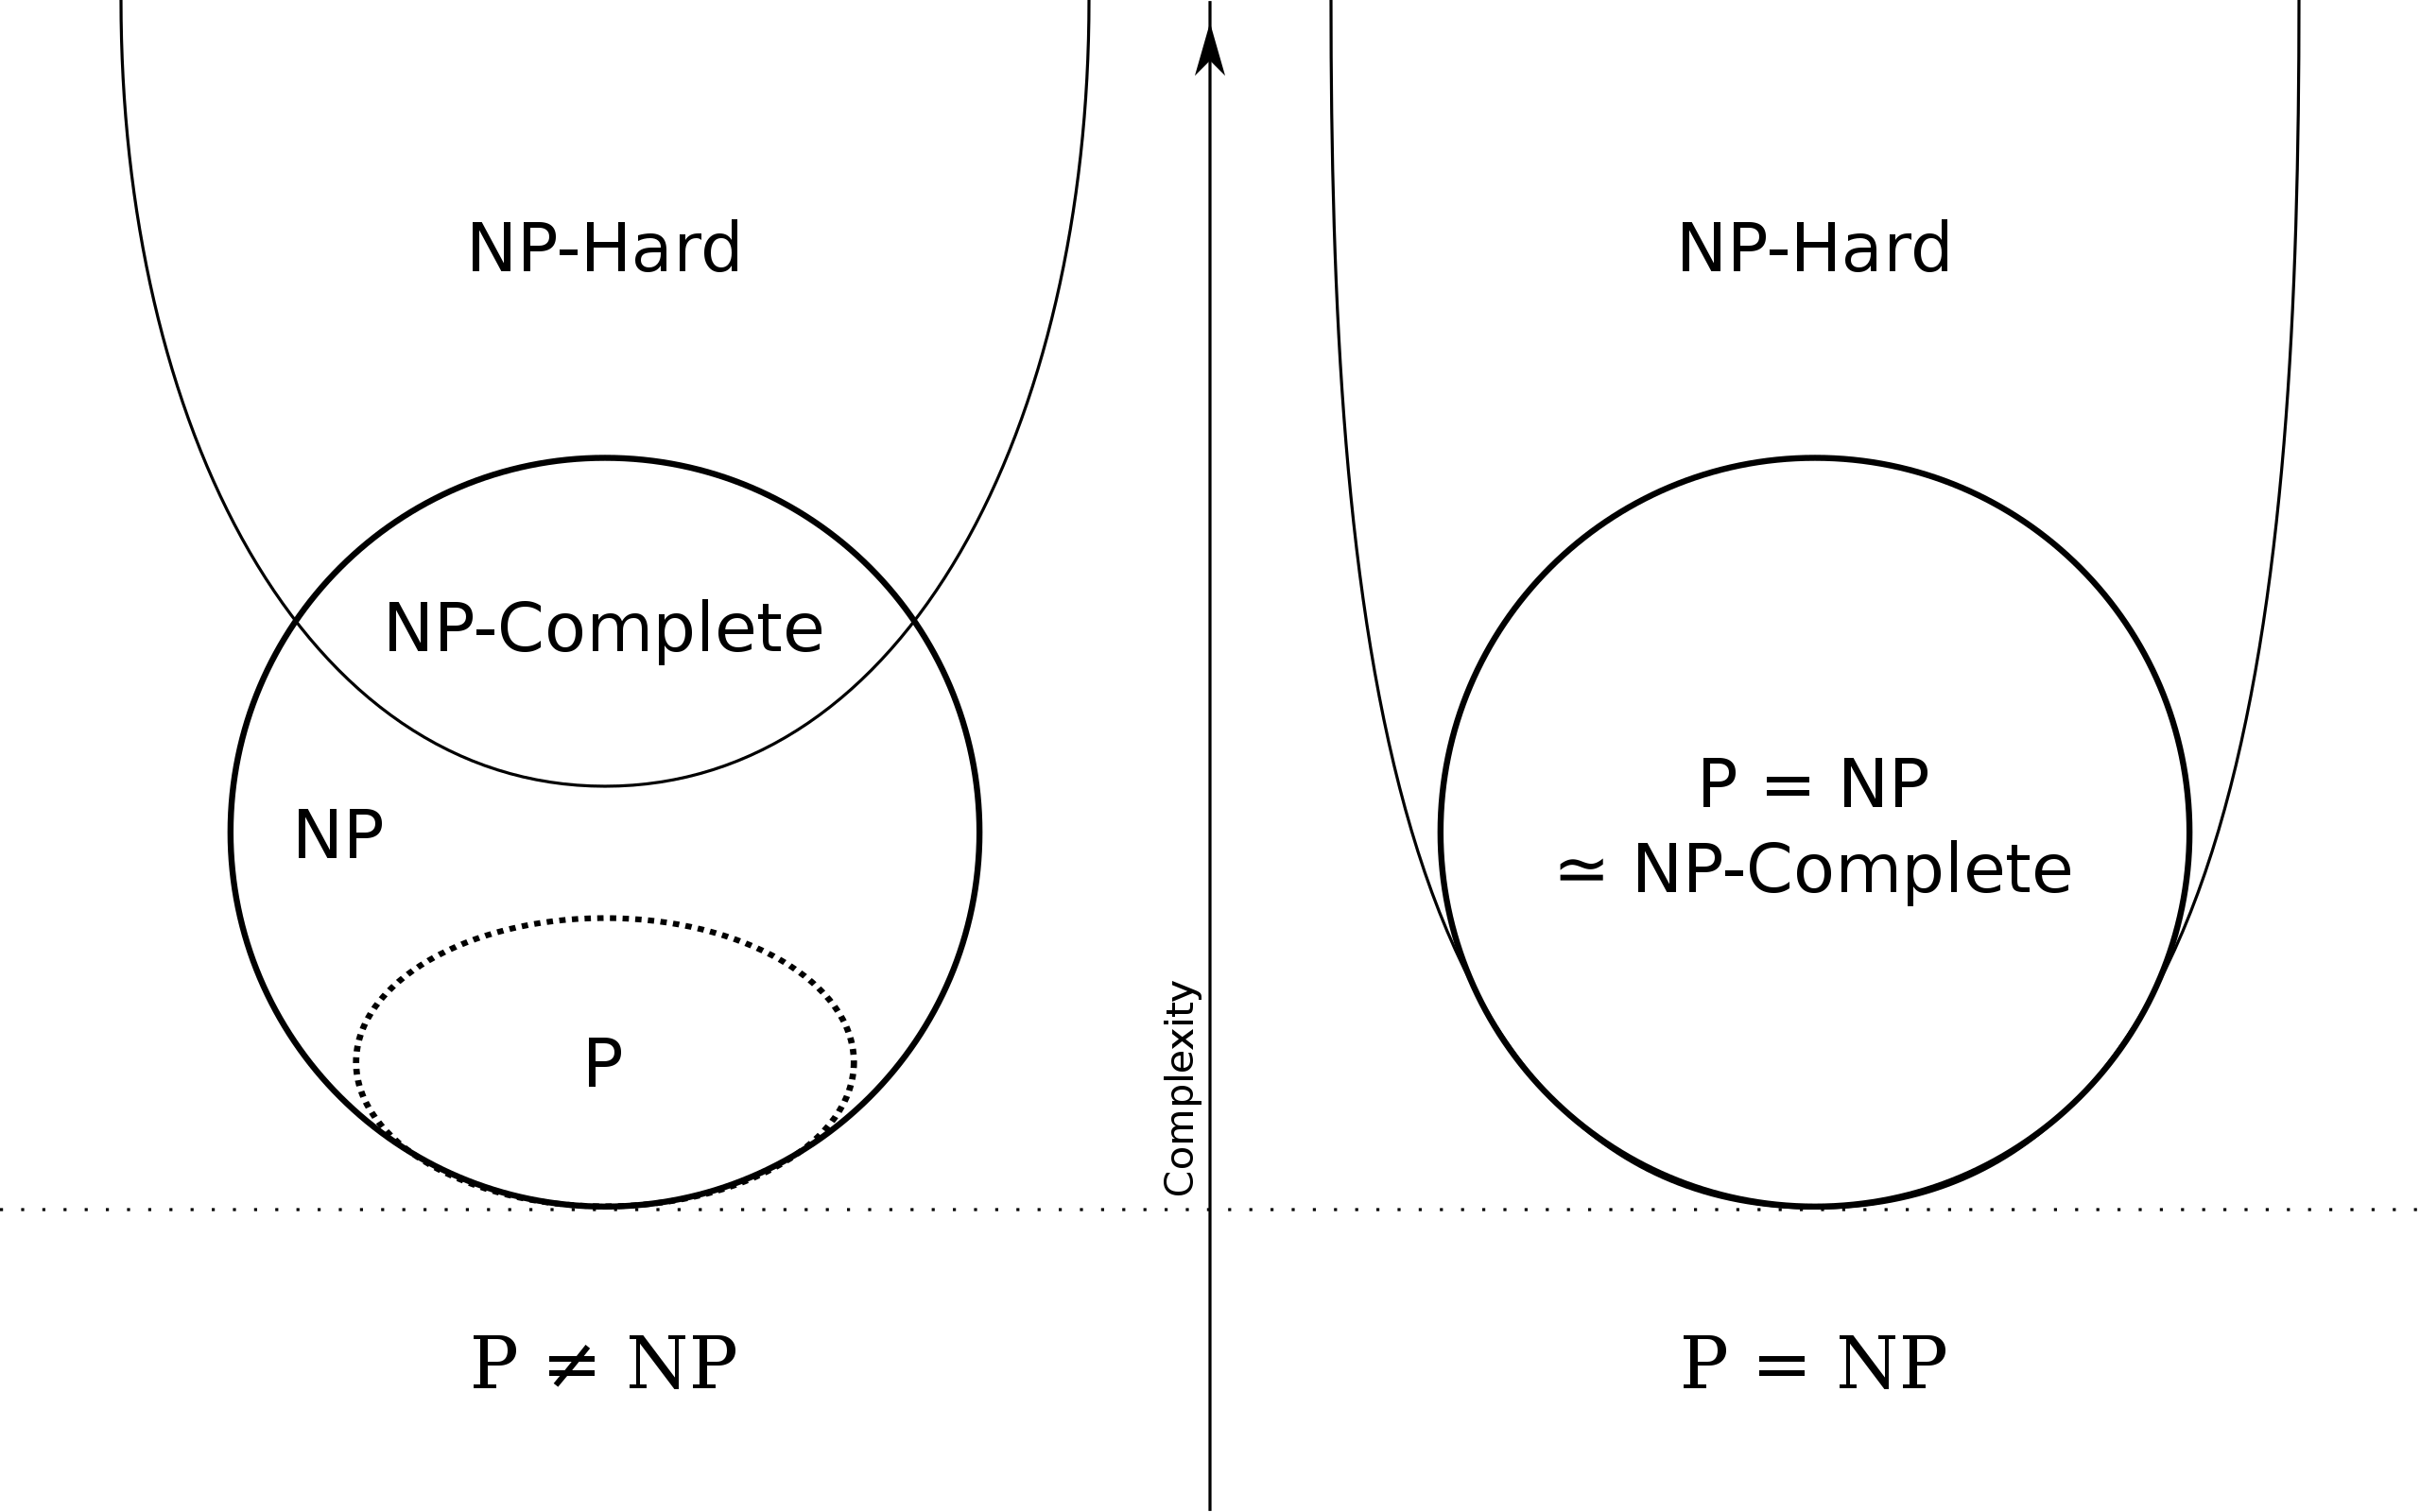
\includegraphics[scale=0.12]{euler_diagram}
    \caption{Diagramme d'Euler sur les classes de complexité}
    \label{fig:euler_diagram}
\end{figure}

\subsection{Classe P}
C'est la classe des problèmes résolus dans un temps polynomial (ou moins) par une machine de Turing déterministe \emph{pour tout instance d'entrée}. Les problèmes de classe P sont considérés comme des problèmes qui sont rapide à résoudre, et par la suite faciles. Quelques problèmes dans la classe P: optimisation linéaire, évaluation d'un circuit et multiplication des entiers.

\subsection{Classe NP}
C'est la classe des problèmes résolus dans un temps polynomial par une machine de Turing non déterministe \emph{pour tout instance d'entrée}. Par contre, une solution donnée peut être vérifiée dans un temps polynomial par une machine de Turing déterministe. En pratique, les ordinateurs actuels sont équivalents à des machines de Turing déterministe. Dans ce contexte, un problème de classe NP ne peut pas être résolu par une machine de Turing déterministe dans un temps polynomial.

Le problème le plus connu dans la classe NP est la factorisation d'un entier en nombres premiers. Trouver les facteurs premiers ne peux pas être trouvé dans un temps polynomiale mais si les facteurs sont données, il est rapide de vérifier si leur produit est bien égale au nombre. C'est la base de la cryptographie moderne.

\subsection{Classe NP-complet}
C'est la classe des problèmes NP mais avec une propriété supplémentaire: tout autre problème en classe NP peut être réduit dans un temps polynomial à un problème NP-complet. Il est important de noter aussi que n'importe quel problème dans NP-difficile peut être réduit dans un temps polynomial à un problème NP-complet. \href{https://fr.wikipedia.org/wiki/21_probl\%C3\%A8mes_NP-complets_de_Karp}{Les 21 problèmes NP-complet de Karp} sont les exemples les plus connus de problèmes NP-complet.

\subsection{Classe NP-difficile}
C'est la classe des problèmes résolus dans un temps polynomial par une machine de Turing non déterministe et une solution donnée ne peut pas être vérifiée dans un temps polynomial par une machine de Turing déterministe. Autrement dit, il n'y a pas de méthode pour rapidement vérifier la solution. Le problème du voyageur de commerce est un problème classé dans NP-difficile.

\subsection{Problème P $\stackrel{?}{=}$ NP}

Vérifier l'égalité P $\stackrel{?}{=}$ NP est une question essentielle dans la théorie de la complexité mais qui n'est pas encore résolue. Pour l'instant, tant qu'il n'y a pas de preuve d'algorithme qui résout un problème NP dans un temps polynomial, on suppose P $\neq$ NP.
\end{document}